\section{Related Work}
\label{sec:related_work}

The following section reviews recent work on modeling discrete data distributions using normalizing flows. 
Specifically, Section~\ref{sec:related_work_dequantization} discusses the concept of \textit{dequantization} to represent ordinal discrete data as a continuous distribution, which is commonly used for normalizing flows trained on image modeling \cite{RealNVP, Glow, Flow++}. 
An alternative, popular generative model for discrete data is the framework of \acfp{VAE} \cite{VAE} that model a lower-bound estimate of the data likelihood. 
Its hybrid versions with a flow-based posterior or prior are reviewed in Section~\ref{sec:related_work_VAE_flow}. 
Additionally, normalizing flows can be directly applied to discrete data by reformulating the change-of-variable formula to discrete inputs, which is presented in Section~\ref{sec:related_work_discrete_flows}.
Finally, Section~\ref{sec:related_work_graph_modeling} reviews recent work on applying normalizing flows to the task of graph modeling.

\subsection{Input Dequantization}
\label{sec:related_work_dequantization}

% A common application and benchmark of normalizing flows has been the modeling and generation of images. Thereby, images are a discretized representation of a real-world scene, as in reality, colors are not limited to discrete pixel values. Directly applying continuous normalizing flows on discrete data will lead to an undesired solution \cite{UriaContPeaks, Theis2015}. As discrete points correspond to delta functions with infinite height in continuous space, the flow would try to fit such delta functions. Therefore, the probability of a value such as $127$ could be close to infinity while $127.1$ has one close to zero. Hence, the likelihood values would be almost meaningless as single data points can reach infinite probabilities.
Applying continuous normalizing flows on discrete data leads to undesired density models where arbitrarily high likelihoods are placed on particular values. This is because discrete data points represent delta peaks in a continuous distribution, and a normalizing flow would place arbitrarily high likelihood to those discrete points making the density function useless \cite{Theis2015, UriaContPeaks}. 
To prevent such degenerated solutions, a common solution is to add a small amount of noise to each discrete value, which is also referred to as dequantization \cite{RealNVP, Flow++, EmielDequantization}. 
Considering $\bm{x}$ as an integer, the dequantized representation $\bm{v}$ can be formulated as $\bm{v}=\bm{x}+\bm{u}$ where $\bm{u}\in[0,1)^D$. 
Thus, the discrete value $1$ is modeled by a distribution over the interval $[1.0, 2.0)$.   \citet{Theis2015} have shown that modeling the dequantized representation, $p_{\text{model}}(\bm{v})$, lower-bounds the modeled discrete distribution $P_{\text{model}}(\bm{x})$, and hence prevents arbitrarily high likelihoods. 
Meanwhile, the flow remains invertible as $\bm{x}+\bm{u}$ constitute disjoint intervals so that each continuous point can be mapped back to exactly one discrete point $\bm{x}$ by finding the next lower whole number for each element $v_i$. 
In summary, modelling the discrete data distribution $P_{\text{data}}(\bm{x})$ by a normalizing flow can be written as:
\begin{eqnarray}
    \label{eqn:related_work_dequantization_uniform}
    % P_{\text{model}}(\bm{x}) = \int_{[0,1)^D} p_{\text{model}}(\bm{x}+\bm{u})\hspace{1mm}d\bm{u} = \E_{\bm{u} \sim [0,1)^D}\left[p_{\text{model}}(\bm{x}+\bm{u})\right] \\
    & & \E_{\bm{x}\sim P_{\text{data}}}\left[\log P_{\text{model}}(\bm{x})\right] \geq \E_{\bm{x}\sim P_{\text{data}}}\E_{\bm{u} \sim [0,1)^D}\left[\log p_{\text{model}}(\bm{x}+\bm{u})\right]
\end{eqnarray}
% following the notation of \citet{Flow++} where $P(x)$ represents the discrete probability distribution, and $p(x)$ the continuous flow-modeled distribution. The vector $\bm{u}$ corresponds to uniform noise which is sampled independently for all $D$ dimensions of the data.

Nevertheless, by representing discrete values as uniform distributions, the flow is required to model unit hypercubes around the data points. This is difficult for smooth transformation to capture and has shown to harm the modeling capacity \cite{EmielDequantization} (see Figure~\ref{fig:related_work_dequantization_techniques}). Dequantization has therefore been extended to more sophisticated, learnable distributions beyond uniform in a variational framework. In particular, the uniform distribution can be replaced by a learned distribution $q(\bm{u}|\bm{x})$ with support over $\bm{u}\in[0,1)^D$ by rewriting Equation~\ref{eqn:related_work_dequantization_uniform} as follows:
\begin{equation}
    \label{eqn:related_work_dequantization_variational}
    % P(\bm{x}) = \int_{[0,1)^D} q(\bm{u}|\bm{x})\frac{p(\bm{x}+\bm{u})}{q(\bm{u}|\bm{x})} d\bm{u} = \E_{\bm{u} \sim q(\bm{u}|\bm{x})}\left[\frac{p(\bm{x}+\bm{u})}{q(\bm{u}|\bm{x})}\right]
    \E_{\bm{x}\sim P_{\text{data}}}\left[\log P_{\text{model}}(\bm{x})\right] \geq \E_{\bm{x}\sim P_{\text{data}}}\E_{\bm{u}\sim q(\cdot|\bm{x})}\left[\log \frac{p_{\text{model}}(\bm{x}+\bm{u})}{q(\bm{u}|\bm{x})}\right]
\end{equation}
The distribution $q(\bm{u}|\bm{x})$ is commonly implemented by a normalizing flow conditioned on the input $\bm{x}$ (i.e. the applied transformations are influenced by $\bm{x}$). 
The constraint of having a support only over the unit hypercube $[0,1)^D$ can be fulfilled by applying a sigmoid activation function on the final output of the normalizing flow. 
Currently, models with variational dequantization like autoregressive models constitute the \acl{SOTA} for flow-based image modeling \cite{VFlow, EmielDequantization}. 

Such dequantization techniques, however, cannot be as simply applied on nominal discrete data where the values represent categories with no intrinsic order. 
Treating these categories as integers for dequantization biases the data to a non-existing order, and consequently makes the modeling task significantly harder.
Therefore, the application of variational dequantization has been mostly limited to ordinal discrete data.

\begin{figure}[t!]
    \centering
    \begin{subfigure}{0.4\textwidth}
        \centering
        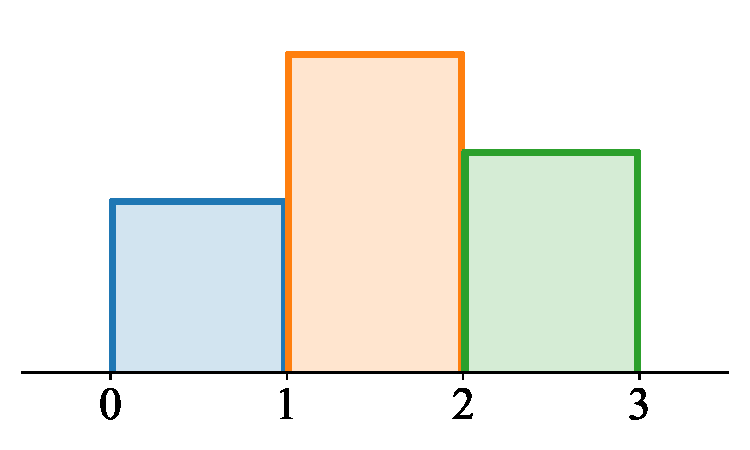
\includegraphics[width=0.65\textwidth]{figures/related_work_figures/dequant.pdf}
        \caption{Uniform dequantization}
    \end{subfigure}
    \begin{subfigure}{0.4\textwidth}
        \centering
        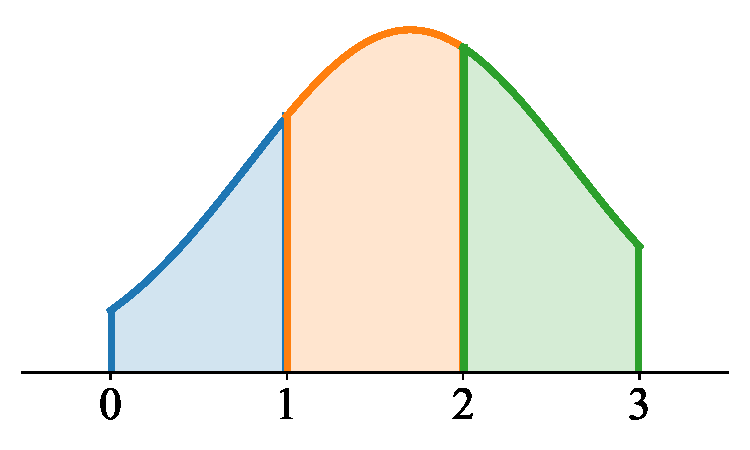
\includegraphics[width=0.65\textwidth]{figures/related_work_figures/var_dequant.pdf}
        \caption{Variational dequantization}
    \end{subfigure}
    \caption[Uniform and variational dequantization]{Visual comparison between (a) uniform and (b) variational dequantization for the integers $0$ (blue), $1$ (orange) and $2$ (green). The continuous representation shows the dequantization distribution of $x+u$ for a single dimension. While the uniform case requires the flow to model sharp edges between integers, variational dequantization allows for more flexible distributions and simplifies the modeling task for the consecutive normalizing flow.}
    \label{fig:related_work_dequantization_techniques}
\end{figure}

%%% - SUBSECTION - %%%
\subsection{Flow-based Variational Auto-Encoders}
\label{sec:related_work_VAE_flow}

In contrast to normalizing flows, \acp{VAE} \cite{VAE} can handle discrete data without additional overhead. This is because the \ac{VAE} framework models the following variational lower bound of the data likelihood, called \ac{ELBO}:
\begin{equation}
    \log p(\bm{x}) \geq \E_{q_{\phi}(\bm{z}|\bm{x})}\left[\log p_{\theta}(\bm{x}|\bm{z}) + \log p_{\theta}(\bm{z}) - \log q_{\phi}(\bm{z}|\bm{x})\right]
\end{equation}
The likelihood $p_{\theta}(\bm{x}|\bm{z})$ represents the decoder (i.e. decoding latent variable $\bm{z}$ to $\bm{x}$), while the (approximate) posterior $q_{\phi}(\bm{z}|\bm{x})$ is the encoder (i.e. encoding $\bm{x}$ into latent variable $\bm{z}$). The difference between the true log-likelihood and the ELBO is the KL divergence between the approximate posterior $q_{\phi}(\bm{z}|\bm{x})$ and the true (unknown) posterior $p_{\theta}(\bm{z}|\bm{x})$: $D_{\text{KL}}(q_{\phi}(\bm{z}|\bm{x})||p_{\theta}(\bm{z}|\bm{x}))$.
Both the encoder and decoder are usually implemented by deep neural networks, which, in comparison to normalizing flows, do not have to be invertible. Thus, a mapping from discrete space to continuous is easily possible by predicting a suitable distribution for $\bm{z}$. 

The prior $p_{\theta}(\bm{z})$ is often assumed to be a standard normal distribution in the \ac{VAE} \cite{VAE} but also other distributions such as Mises-Fisher on hyperspherical space \cite{VAEHyperspherical} or mixture-based approaches \cite{VAESemiSupervised, VampPrior} have been proposed. The output of the encoder $q_{\phi}(\bm{z}|\bm{x})$ is usually designed to fit the prior distribution. For a Gaussian prior with diagonal covariance, the encoder predicts a mean and variance per latent dimension. This allows an efficient computation of the KL divergence between prior and encoder, but limits the flexibility of the encoder which is needed to accurately fit the true posterior $p_{\theta}(\bm{z}|\bm{x})$. One approach for increasing flexibility is applying a normalizing flow on top of the output of the encoder \cite{InverseAutoregressiveFlows}. Those flow transformations are parameterized by the features of the encoder, to allow simpler, input-dependent transformations. Figure~\ref{fig:related_work_VAE_flow_hybrids_1} visualizes the approach. The usage of various kinds of normalizing flows has been explored in the setting of a \ac{VAE}, including inverse autoregressive flows \cite{InverseAutoregressiveFlows} and Sylvester normalizing flows \cite{SylvesterNF}, a generalization of planar flows.

\begin{figure}[t!]
    \centering
    \begin{subfigure}{0.53\textwidth}
        \centering\vspace{8mm}
        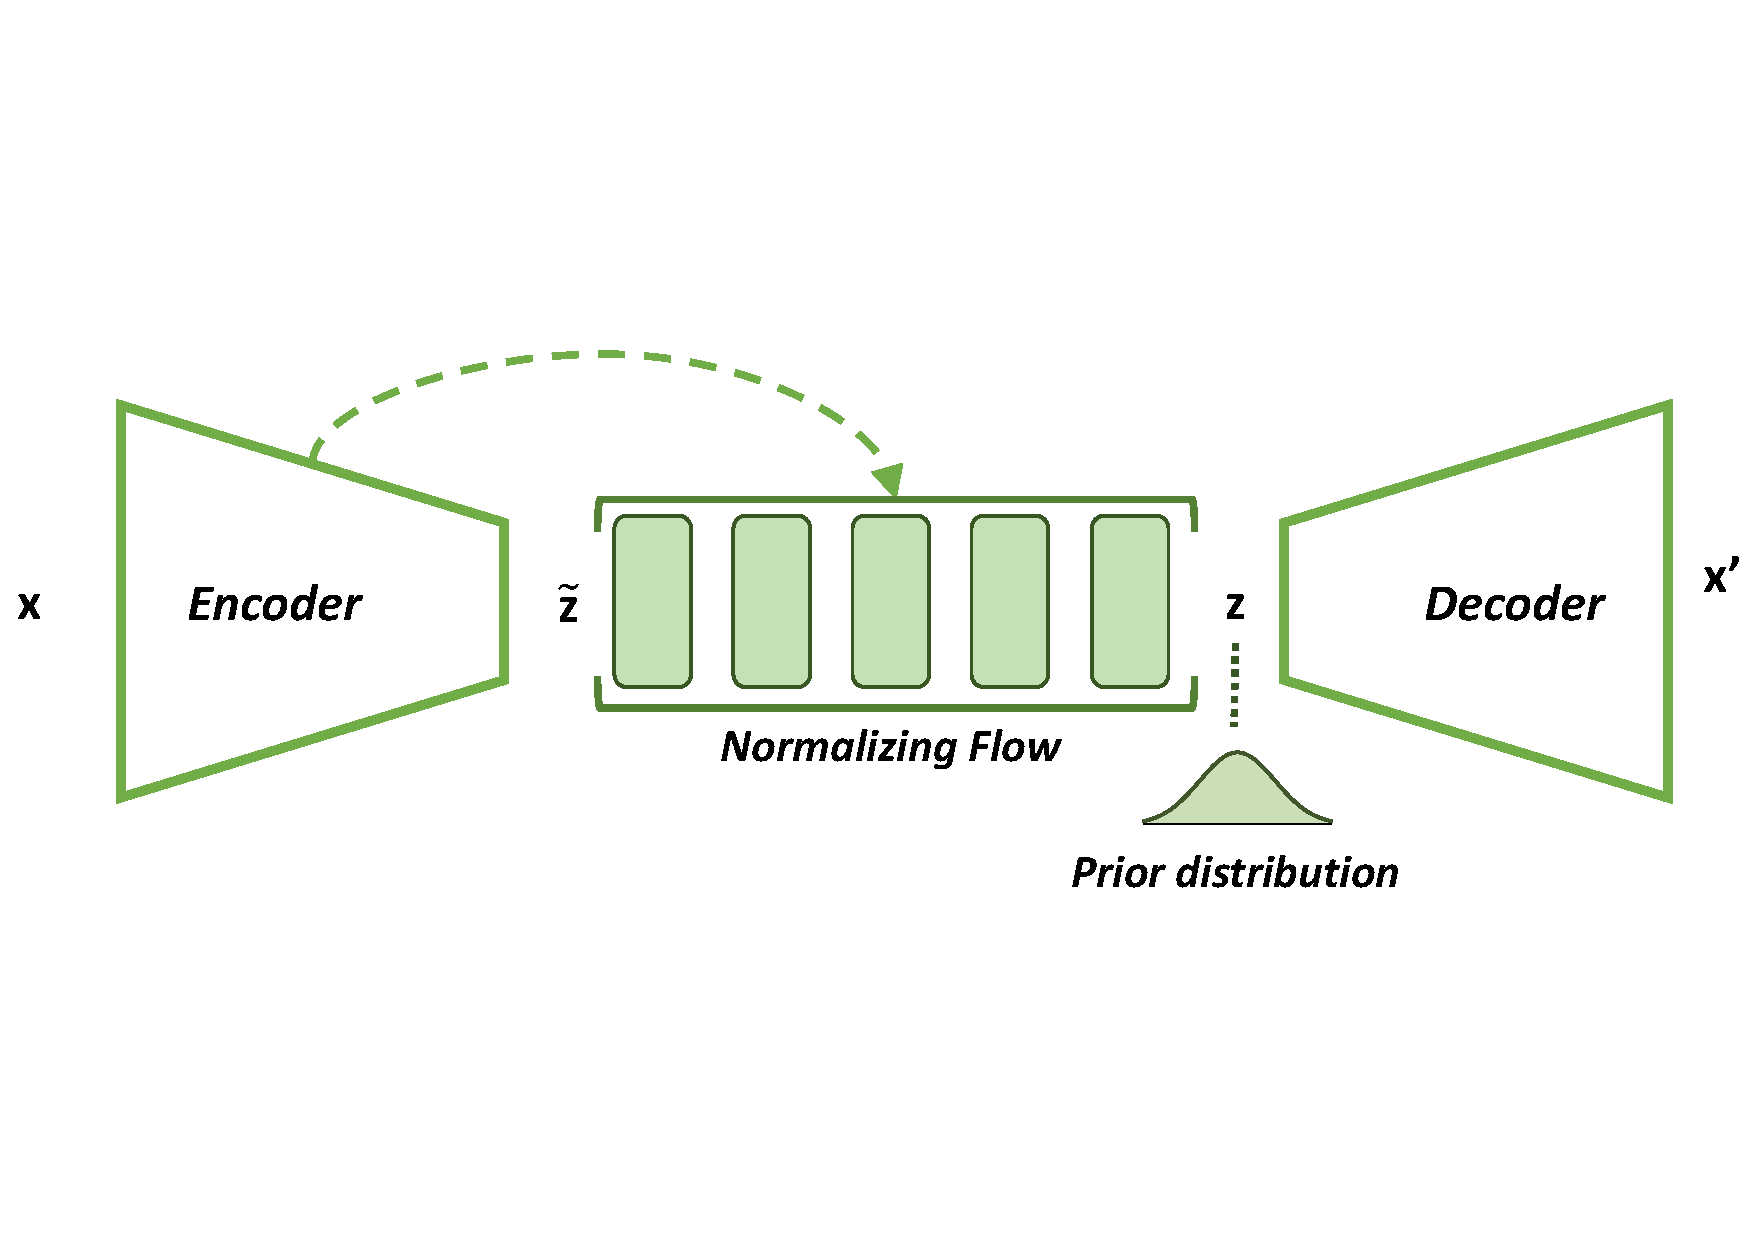
\includegraphics[width=\linewidth]{figures/related_work_figures/VAE_Flow_1.pdf}\vspace{8mm}
        \caption{Flow-based encoder}
        \label{fig:related_work_VAE_flow_hybrids_1}
    \end{subfigure} \hspace{10mm}
    \begin{subfigure}{0.39\textwidth}
        \centering
        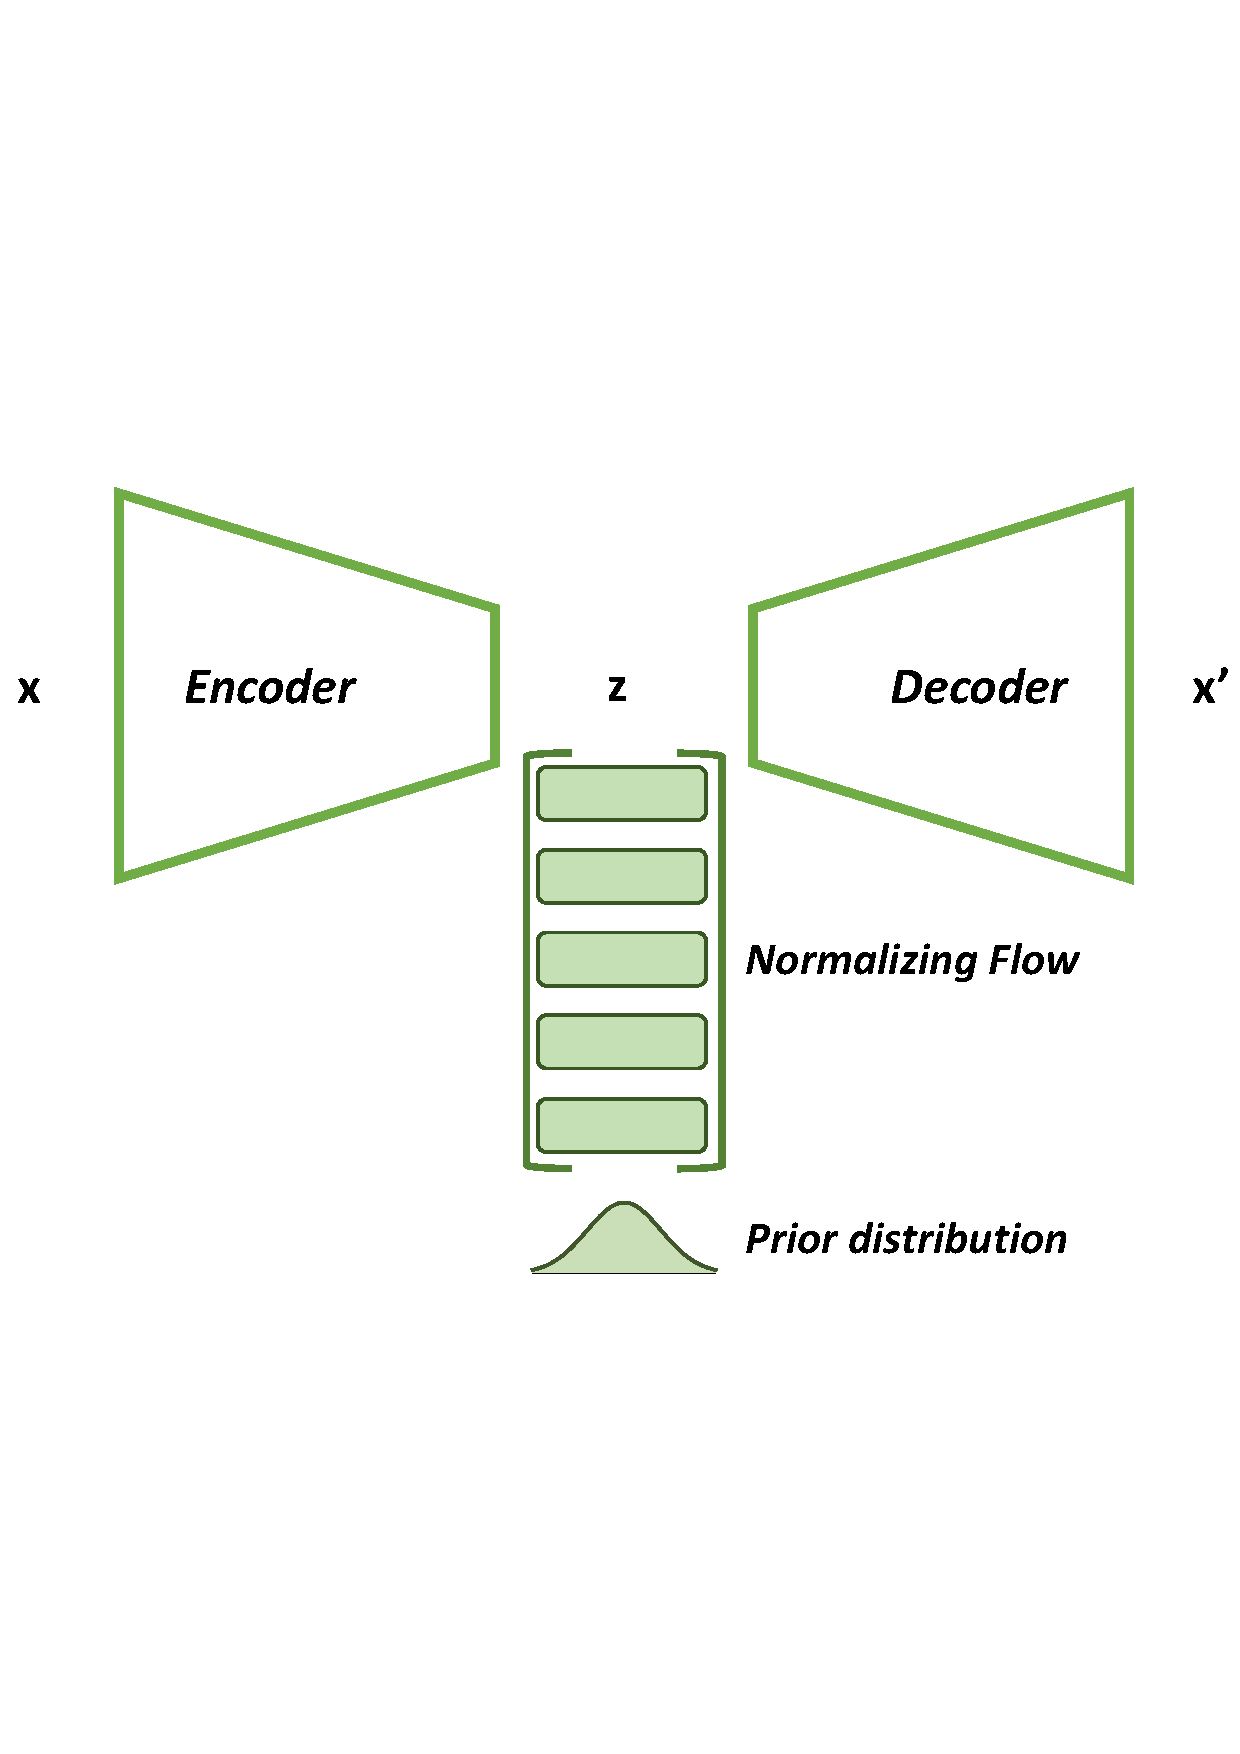
\includegraphics[width=\linewidth]{figures/related_work_figures/VAE_Flow_2.pdf}
        \caption{Flow-based prior}
        \label{fig:related_work_VAE_flow_hybrids_2}
    \end{subfigure}
    \caption[Hybrid model variants for combining VAEs with normalizing flows]{Hybrid model variants for combining \ac{VAE} with normalizing flows. (a) The encoder's distribution can be extended by applying a normalizing flow on top of a simpler output distribution $q_{\phi}(\bm{z}'|\bm{x})$. Features from the encoder parameterize the flow. The output of the flow, representing $\bm{z}$, is trained to follow the prior distribution $p(\bm{z})$. (b) The prior $p(\bm{z})$ can itself be a normalizing flow allowing a more flexible prior distribution. The encoder and decoder are usually smaller in this case as the complexity is moved into the prior.}
    \label{fig:related_work_VAE_flow_hybrids}
\end{figure}

A second approach, called Latent Normalizing Flows \citet{SemiDiscreteNFSequence}, is to model the prior $p(\bm{z})$ by a normalizing flow instead (see Figure~\ref{fig:related_work_VAE_flow_hybrids_2}). 
In this setup, the main modeling complexity is moved into the normalizing flow while the encoder and decoder networks are usually simplified. 
As a result, the KL divergence between the approximate and true posterior is expected to be considerably lower and pushes the evidence lower bound closer to the true likelihood. 
This motivation was verified by experiments of \citet{SemiDiscreteNFSequence} where the reconstruction loss was close to zero while the prior likelihood dominated the objective. 
Although the flow requires $\bm{z}$ to be continuous, the input $\bm{x}$ can be discrete. 
Nevertheless, experiments on language modeling showed that even a 5 layer autoregressive flow was not able to meet the single-layer RNN baseline. 
The encoder and decoder were both modeled by a two-layer bidirectional LSTM \cite{LSTM}.
This suggests that the added complexity of the encoder and decoder actually harms the modeling capability of the normalizing flow, and we verify this issue by experiments in Section~\ref{sec:experiments_language_modeling}.
% \TODO{This part needs to be clear and convincing. Currently it is not...}

% Nevertheless, the \ac{VAE} framework only models a lower bound instead of an exact likelihood estimate as in the standard setup for normalizing flows. Furthermore, the decoder can suffer from posterior collapse ignoring the latent code \cite{VAEPosteriorCollapse}. This has even been the case for shallow decoder networks used by \cite{SemiDiscreteNFSequence}.

%%% - SUBSECTION - %%%
\subsection{Discrete Normalizing Flows}
\label{sec:related_work_discrete_flows}

Recent works by \citet{TranDiscreteFlows}, \citet{IntegerNF} and \citet{IDF++} have explored the approach of applying normalizing flows directly on discrete data. In particular, the rule of change of variable for an invertible function $f$ can be formulated on discrete input data as follows:
\begin{equation}
    \label{eqn:change_of_variable_discrete}
    p(\bm{z}'=z') = p(\bm{z}=f^{-1}\left(z'\right))
\end{equation}
Note that in contrast to Equation~\ref{eqn:related_work_change_of_variables}, the discrete formula does not have a log-determinant Jacobian which takes the volume change into account. This is because in a discrete space there exists no volume which could be modified. 
Furthermore, two inputs cannot be mapped to the same output as otherwise, the function is not invertible anymore. 
Hence, the determinant of the Jacobian will always be one.

Designing the invertible function $f$ can be done similarly as for the continuous case. For instance, \citet{IntegerNF} proposed to discretize the transformation by rounding the additive term of the affine coupling layer:
\begin{equation}
    \bm{z}^{(k)}_{i} = \bm{z}^{(k-1)}_{i} + \big\lfloor\bm{\mu}_{\theta,i}\big\rceil
\end{equation}
where $\lfloor\cdot\rceil$ denotes the rounding operator to the nearest integer. 
The transformation can be defined as $f:\mathbb{Z}^{d}\to\mathbb{Z}^{d}$. 
Since the rounding operator is similar to a step function and has zero gradients for almost any input, a straight-through estimator \cite{STEGradientEstimator} is applied.
This estimator effectively skips the rounding operator during backpropagation and assumes a unit gradient everywhere: $\nabla_{x}\lfloor x\rceil = 1$.
However, note that this introduces gradient bias as backpropagation is not performed on the ``true'' gradients. 

The coupling layers introduced by \citet{IntegerNF} work well on integers, but in the case of categorical variables, the input space is bounded to a finite, discrete set on which the transformations have to operate. 
For this setup, \citet{TranDiscreteFlows} proposed the following affine coupling layer:
\begin{equation}
    \bm{z}^{(k)}_{i} = (\bm{\mu}_{\theta,i} + \bm{\sigma}_{\theta,i} \odot \bm{z}^{(k-1)}_i) \hspace{-2mm}\mod{M}
\end{equation}
where $\bm{\mu}_{\theta,i}$ and $\bm{\sigma}_{\theta,i}$ are functions with discrete outputs parameterized by $\theta$, and $\bm{\mu}_{\theta,i}, \bm{\sigma}_{\theta,i}, \bm{z}^{(k-1)}_{i} \in \llbracket0\mathrel{{.}\,{.}}\nobreak M-1\rrbracket$ where $M$ denotes the number of categories in the discrete distribution.
The modulo operator ensures that the output space is in the same finite, discrete set as the input. 
For the scaling transformation to be invertible, $\bm{\sigma}_{\theta,i}$ and $M$ have to be coprime. 
As $M$ is usually fixed by the task and/or input distribution, $\bm{\sigma}_{\theta,i}$ has been set to 1 for simplicity in most experiments. 

To predict the discrete transformation parameters $\bm{\mu}_{\theta,i}$ and $\bm{\sigma}_{\theta,i}$, \citet{TranDiscreteFlows} proposed to use a standard softmax output and discretize it by taking the argmax over logits. 
However, to maintain a fully differentiable architecture, the argmax operator is replaced by the Gumbel softmax \cite{GumbelSoftmax1, GumbelSoftmax2} using a straight-through estimator \cite{STEGradientEstimator} during backpropagation:
\begin{equation}
    \frac{\partial \bm{\mu}_{\theta,i}}{\partial \theta} \approx \frac{\partial}{\partial \theta} \text{softmax}\left(\frac{\theta}{\tau}\right)
\end{equation}
The temperature parameter $\tau$ controls the trade-off between bias of the gradient estimator and vanishing gradients. 
If $\tau\to 0$, the softmax becomes an argmax, so that the bias is reduced to zero while the gradients vanish and harm learning. 
When $\tau$ is large, the bias of the gradient estimator becomes large due to the considerable difference between the argmax and softmax. 
Keeping the gradient estimator bias low is especially crucial for deep normalizing flows as the bias can aggregate over layers and destabilize the training \cite{EmielDequantization}.

In experiments on the task of language modeling, discrete normalizing flows have shown to perform on par with autoregressive models such as LSTM while allowing a fully parallelized generation process. 
Moreover, discrete flows outperformed the flow-based \ac{VAE} approach by \citet{SemiDiscreteNFSequence}. % , underlining that operating on a discrete space is not a drawback for a normalizing flow
Nevertheless, the argmax approximations prevent the number of categories to be scaled up to more than 200 as otherwise, the bias of estimator becomes too large \cite{GumbelSoftmax1, GumbelSoftmax2}.

Despite the success of discrete flows on the experiments deducted by \citet{TranDiscreteFlows}, several works have pointed out the limitations of such flows besides gradient approximation \cite{SemiDiscreteNFSequence, NormalizingFlowsOverview2, IDF++}. 
In particular, due to the invertibility constraint in Equation~\ref{eqn:change_of_variable_discrete}, transformations in discrete flows can only model permutations of the input set \cite{SemiDiscreteNFSequence}.
This significantly limits the modeling capability in low-dimensional spaces and prevents the flow from learning arbitrary distribution with factorized base distributions as it is the case for continuous flows.
For example, suppose we have the following distribution over $\bm{x}\in\{0,1\}^{2}$:
\begin{table*}[ht!]
    \centering
    \begin{tabular}{ccc}
         & $x_2=0$ & $x_2=1$ \\
         \midrule
         $x_1=0$ & $0.1$ & $0.2$ \\
         $x_1=1$ & $0.3$ & $0.4$ \\
         \bottomrule
    \end{tabular}
\end{table*}

Within the $4!$ possible permutations, there exists no invertible transformation from $\bm{x}$ to $\bm{z}\in\{0,1\}^{2}$ such that $p_z(\bm{z})$ can be expressed as by two factorized base distributions: $p_x(\bm{x})=p_z(\bm{z})=p_z(z_1)p_z(z_2)$.
Although \citet{IDF++} argue that by expanding the domain of $\bm{x}$ and $\bm{z}$ to $\{0,1,2,3\}^{2}$, the probability distribution can be modeled by a discrete flow, this only generalizes by expanding the domain to $M^{d}$ elements which is infeasible for real-world data like text.
Therefore, those flows have to rely on strong base distributions such as autoregressive ones, which inherently slow down sampling.
On the other hand, normalizing flows on continuous data can model any input distribution with the requirement of using sufficiently complex transformations \cite{NormalizingFlowsOverview, NormalizingFlowsOverview2}. 


\subsection{Graph modeling}
\label{sec:related_work_graph_modeling}

\begin{figure}[b!]
    \centering
    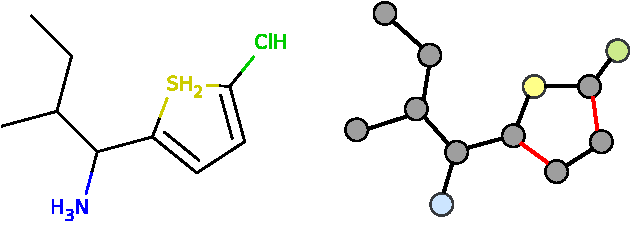
\includegraphics[width=0.65\textwidth]{figures/related_work_figures/molecule_graph.pdf}
    \caption[Visualization of molecule graph]{In graph-based molecule generation, the chemical representation (left) is translated into a graph (right) by encoding atoms as nodes and bonds as edges. Node and edge categories are visualized by different colors. The task is to model a distribution of valid graphs which is coherently difficult as the models have to consider edges between any pairs of nodes. Molecule taken from the Zinc250k dataset \cite{Zinc250k}.}
    \label{fig:related_work_graph_molecule}
\end{figure}

Modeling and generating graphs is a crucial application in areas such as biology and chemistry, and deep learning approaches have recently gained interest in such tasks \cite{GraphRNN, GraphOverview1, GraphOverview2, GraphAF}.
A graph $\mathcal{G}=(V,E)$ is defined by a set of vertices or nodes $V$, and a set of tuples representing edges $E$ between vertices. 
A common alternative representation of the edges is the adjacency matrix whose elements indicate whether a pair of nodes is connected by an edge or not.
Both the nodes and edges can have attributes that are often categorical and need to be predicted as well besides the overall graph structure.
The first generation models on graphs have been autoregressive \cite{GraphRNNAttention, GraphRNN, MolecularRNN}, generating nodes and edges in sequential order. 
While being efficient in memory, they are slow in sampling as the generation time scales quadratically with the number of nodes (for $N$ nodes, there are $N(N-1)/2$ edges to predict).

However, a considerable drawback of autoregressive models on graphs is that they assume an order in the set of nodes although the nodes are not a sequence. 
Permuting the nodes in the set while adjusting the edges accordingly represents the exact same graph.
Therefore, a generative model should ideally be permutation invariant concerning the order in the set as well to automatically assign the same likelihood to each ordering of a graph. 
Nonetheless, autoregressive models are sensitive to the order assigning the same graph with different orderings different likelihood values.
Furthermore, previous work has shown that introducing an order to an actually unordered set can lead to a strong bias and harms the performance \cite{OrderMatters}.

Normalizing flows, on the other hand, can perform generation in parallel allowing them to build a permutation invariant density model.
The first application of normalizing flows for graph generation was introduced by \citet{GraphNF}, where a flow models the latent node representations of a pretrained autoencoder. 
While the proposed flow is permutation invariant, the model does not support node or edge attributes.
Recent works of GraphNVP \cite{GraphNVP} and GraphAF \cite{GraphAF} showed applications on molecule generation where nodes represent atoms and edges different types of bonds between the atoms (see Figure~\ref{fig:related_work_graph_molecule}). 

GraphNVP consists of two separate flows, one for modeling the adjacency matrix and a second for modeling the node types. 
Although allowing parallel generation, the model is sensitive to the node order due to two design choices.
Firstly, the coupling layers in GraphNVP transform the latent variables of a single node, which is decided based on an assumed order, while using all others as input.
Hence, permuting the nodes represents a different graph for the model. 
Secondly, the feature networks in the coupling layers are multi-layer perceptrons that flatten the adjacency matrix into a vector.
Thus, the predicted transformation parameters are sensitive to the node order and fixed to a specific graph size (the model cannot generate graphs larger than in the training set).
In comparison, GraphAF combines autoregressive models and normalizing flows by applying autoregressive flows on the graph structure. 
Although having the same drawbacks as autoregressive models, it provides a latent space which can be used for tasks like drug discovery \cite{MolecularRNN, GraphAF} and outperforms GraphNVP by a considerable margin.

To embed the discrete, categorical node and edge attributes into continuous space, both flows use standard uniform dequantization on a one-hot representation of its categories.
In this work, we use a variational inference framework instead for the mapping to continuous values. 
Using this representation, we can design a fully permutation-invariant normalizing flow on graphs, called GraphCNF, which assigns an equal likelihood to any permutation of the nodes.


Variational autoencoders have also been proposed for latent-based graph generation \cite{GraphVAE, GraphVAEConstrained, GraphVAEConstrained2, JunctionTreeVAE}. 
Usually, an encoder transforms the discrete graph structure into latent Gaussian variables of fixed size, based on which a decoder reconstructs the graph by predicting the probability of each edge for a fully connected graph. 
To allow the decoder to predict any order of nodes and edges, the reconstruction loss is based on a graph matching algorithm between the input and output.
As this matching can be expensive to compute and is non-differentiable, most recent work has focused on autoregressive decoders that are sensitive to node orders \cite{JunctionTreeVAE, GraphVAEConstrained2}.
% they model a lower bound of the true likelihood.%


% \subsubsection{Review of related work}
% \label{sec:experiments_graph_generation_related_work}

% The first generation models on graphs have been autoregressive. \citet{GraphRNN} introduced GraphRNN, which generates nodes and edges in sequential order. At each inference step, a node is sampled based on the current subgraph structure. Afterward, the edges of the generated node with any other node are created, which is again performed autoregressively. Multiple variants of this model have been proposed, mostly focusing on increasing its expressiveness \cite{MolecularRNN} or memory efficiency to scale up to graphs with thousands of nodes \cite{GraphAttentionNetwork}. However, one of its limitations is the slow generation as it scales with $\mathcal{O}(N^2)$ where $N$ is the number of nodes.

% For faster generation, \citet{GraphVAE} proposed to use \acl{VAE}s on graphs. Specifically, an encoder transforms the discrete graph structure into latent Gaussian variables of fixed size. Based on this latent representation, a decoder reconstructs the graph by predicting the probability of each edge for a fully connected graph. To allow the decoder to predict any order of nodes and edges, the reconstruction loss is based on a graph matching algorithm.

% Applying normalizing flows for the task of graph generation has first been introduced by \citet{GraphNF}. Their approach consists of two steps, of which the first is to train a standard autoencoder on reconstructing graphs. Each node is encoded to an arbitrary feature vector, and for decoding the adjacency matrix, the cosine similarity is used between those vectors. The second step is to learn the distribution of the encoded node feature vectors by a normalizing flow assuming a fully connected graph in the coupling layers. Note that this approach focused on plain graphs without node or edge properties.

% \citet{GraphNVP} extended this approach solely using a normalizing flow to learn a mapping from the graph to latent space. Their model, called GraphNVP, applies coupling layers on node representations which are based on standard dequantization as used in images \cite{RealNVP}. The layers use a \ac{RGCN} \cite{RGCN} based on the adjacency matrix to be permutation invariant. In a second step, the adjacency matrix itself is transformed into a latent space. However, each row of the adjacency matrix is transformed sequentially increasing the number of flows to 38 and breaking the invariance.

% In a similar manner, \citet{GraphAF} uses an autoregressive flow to generate new molecule graphs. Combining the ideas of GraphRNN and GraphNVP

% \begin{itemize}
%     \item \citet{GraphRNN} (Graph RNN): Recurrent Neural Networks trained to generate graphs. Efficient in-memory usage compared to one-shot approaches, variants of this model can generate large graphs up to thousands of nodes \cite{GraphRNNAttention}.\\
%     \textit{Limitations}: Autoregressive although there is no clear ordering in a graph, and slow in generation
%     \item \citet{GraphNF} (Graph Normalizing Flow): First normalizing flow on graphs. It is build up by a (slightly noisy) auto-encoder, and on its output, a normalizing flow is trained. Training is a two-step process (first train auto-encoder, afterward train flow). \\
%     \textit{Limitations}: Does not consider node- and edge-types. Only predicts a binary adjacency matrix with no node specification. NF in general limit the size of the graph due to its one-shot sampling
%     \item \citet{GraphNVP} (GraphNVP): Graph normalizing flows in the context of molecule generation. Predicts the first adjacency matrix, and uses it to predict the node types. A row-mask is used in the coupling layers.\\
%     \textit{Limitations}: Not permutation invariant, uses simple dequantization and is almost autoregressive for the adjacency matrix and node prediction (one row at a time, overall 38 flows for adjacency matrix).
%     \item \citet{GraphAF} (GraphAF): Combines RNN and Flows to an autoregressive graph normalizing flow. Uses a breadth-first search to determine the (unique) ordering of the nodes. Current \ac{SOTA} on molecule generation.\\
%     \textit{Limitations}: Autoregressive, uses simple dequantization and very task specific 
% \end{itemize}